\documentclass[a4paper,10pt]{article}

\usepackage[utf8]{inputenc}
\usepackage{amsmath, amssymb, hyperref, multirow, dot2texi}

\usepackage{tikz}
\usetikzlibrary{shapes, arrows}

% Title Page
\title{}
\author{}

\parskip = 8pt
\setlength{\parindent}{0pt}
\DeclareMathOperator{\Dir}{Dir}
\DeclareMathOperator{\Mult}{Mult}
\renewcommand{\phi}{\varphi}
\renewcommand{\epsilon}{\varepsilon}
\newcommand{\eps}{\epsilon}

\begin{document}

\section{Introduction} % Problem Formulation

In recent years, several successes have been booked for applying semantic analysis on user comments of movies.
In this report we use those same techniques, but apply them to plot summaries of movies to try and estimate the score these movies are rated with on the popular online movie database IMDb.
These user-written texts roughly describe what happens in a particular movie and may therefore be an indication of the score, which is also calculated from user submitted data.

This project is part of the Natural Language Processing course of the UvA from Fall 2014.

\section{Models}
In this section we describe the extended topic based model we used.
It is taken from \cite{dfsdf}.

The generative version of LDA is as follows:
\begin{enumerate}
  \item Draw topic proportions $\theta \mid \alpha \sim \Dir(\alpha)$.
  \item For each word:
  \begin{enumerate}
    \item Draw topic assignment $z_n \mid \theta \sim \Mult(\theta)$.
    \item Draw word $w_n \mid z_n, \beta_{1:K} \sim \Mult(\beta_{zn})$.
  \end{enumerate}
\end{enumerate}
Its graphical representation can be seen in Figure~\ref{fig:LDA}.

\begin{figure}[ht!]
  \centering
  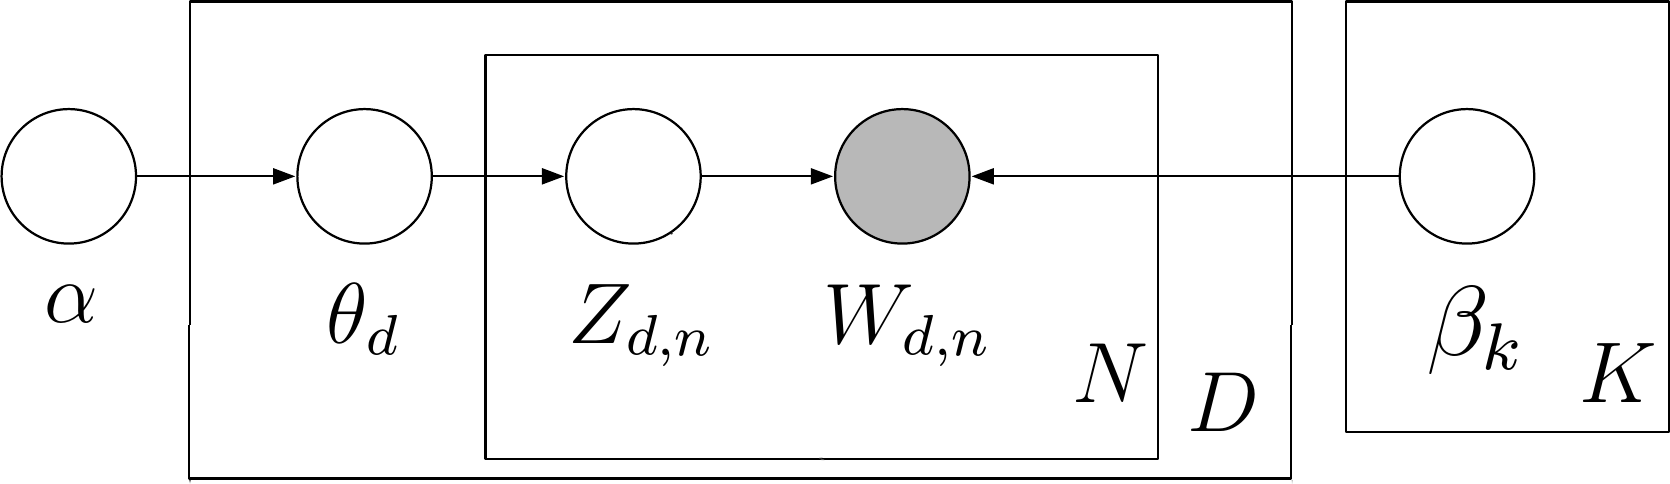
\includegraphics[width=\textwidth]{LDA.png}
  \label{fig:LDA}
  \caption{A graphical representation of traditional LDA model.}
\end{figure}

We however, use the an extended version of LDA, which makes use of the given scores. 
Because of this, a third step is added to the generative process:

\begin{enumerate}
  \item Draw topic proportions $\theta \mid \alpha \sim \Dir(\alpha)$.
  \item For each word:
  \begin{enumerate}
    \item Draw topic assignment $z_n \mid \theta \sim \Mult(\theta)$.
    \item Draw word $w_n \mid z_n, \beta_{1:K} \sim \Mult(\beta_{zn})$.
  \end{enumerate}
  \item[3.] Draw response variable $y \mid z_{1:N}, \eta, \sigma^2 \sim \mathcal{N}(\eta^\top \bar{z}, \sigma^2)$.
\end{enumerate}

This version can be called supervised LDA or SLDA.
Its graphical representation can be seen in Figure~\ref{fig:SLDA}.

\begin{figure}[ht!]
  \centering
  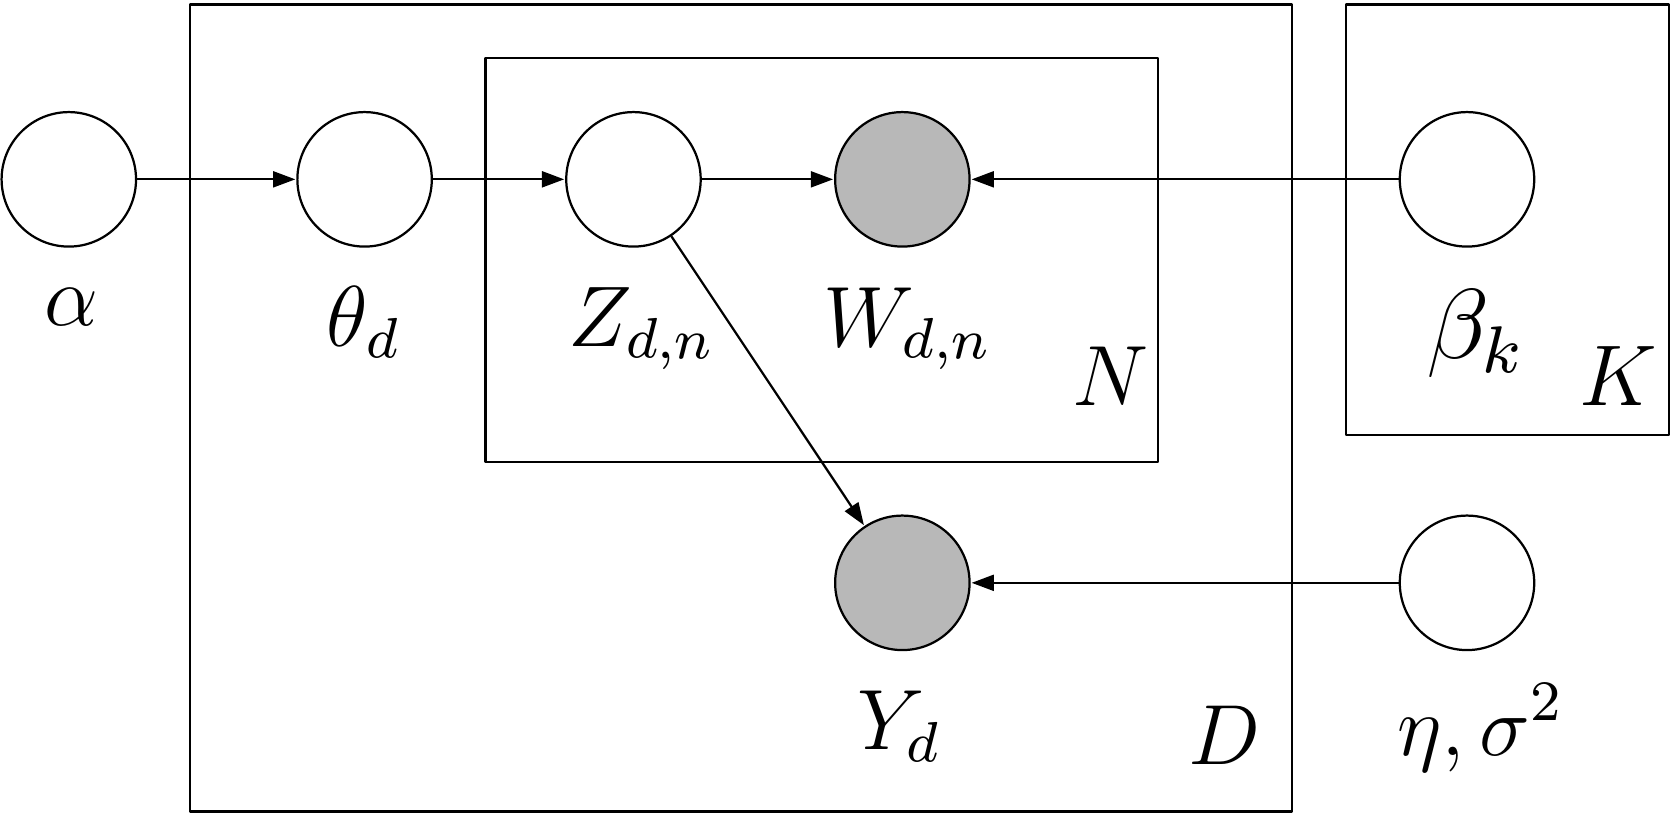
\includegraphics[width=\textwidth]{SLDA.png}
  \label{fig:SLDA}
  \caption{A graphical representation of our modified LDA model.}
\end{figure}

\section{Approach}
(I took this straight from the photo Francesco sent.)
\begin{equation}
  P(\theta, s, z, p,  W\mid \alpha, \beta) = \prod_{d} \Dir(\varphi_d \mid \beta)
\end{equation}
\[\left[ \prod_{d} \Dir(\theta_d \mid \alpha) \prod_d \Mult(\phi_d \mid \theta_d )\Mult(w_d \mid \phi_d)\right]\]
\[\int_{\phi_0}\int_{\phi_1}\dots \int_{\phi_k} P(\theta, s, z, \phi, W \mid \alpha, \beta, \eta, \sigma)\]
\[=\left[ \prod_k \Dir(\phi_k \mid \beta) \right] \left[ \prod_d \Dir(\theta_d \mid \alpha) \mathcal{N}(\eta^\top \bar{z}_d, \sigma) \prod_i^{N_d} \Mult(z) \right]\]
\[\times \left[  \prod_d \prod_i^{N_d} \Mult(w_{di} \mid \phi_{z_d})\right] \rightarrow \prod_d \prod_w \prod_k \left[ \Mult(w \mid \phi_k)^{N_{dk}}\right]\]
\[P(\theta, s, z, w \mid \alpha, \beta, \eta, \sigma) = \left[ \prod_k \int_{\phi_k} \Dir(\phi_k \mid \beta) \prod_d \prod_w \left[ \Mult(w \mid \phi_k)^{N_{dk}}\right] \right]\]
\[ = \left[ \prod_d \Dir(\theta_d \mid \alpha) \mathcal{N}(s_d \mid \eta^\top \bar{z}_d, \sigma) \prod_i^N \Mult(z_{di} \mid \theta_d) \right]\]
\[\times \left[ \prod_k \frac{\Gamma(\beta) \Gamma(W\beta)}{\Gamma(N_k + W\beta)} \prod_w \frac{\Gamma(N_{kw}+\beta)}{\Gamma(\beta)}\right]\]

{next page}

\[P(s, z, w \mid\alpha, \beta, \eta, \sigma) = \]
\[\left[ \prod_k \frac{W\beta}{\Gamma(\beta)^W \Gamma(N_k + W\beta)} \prod_w \Gamma(N_{kw} + \beta)\right]\]
\[\times \left[\prod_d \mathcal{N}(s_d \mid \eta^\top \bar{z}_d, \sigma) \frac{\Gamma(K\alpha)}{\Gamma(\alpha)^K\Gamma(N_d + K \alpha)}\right.\]
\[\left.\times \prod_k \Gamma(N_{dk} + \alpha)\right]\]
%\[P(z \mid s, w, \alpha, \beta, \eta, \sigma) = \frac{P(s, w \mid z) P(z)}{P(}\]

\[P(z\mid s, W, \dots) \overset{\text{Bayes}}{=} \frac{P(s,w \mid z, \dots) P(z\mid \dots)}{P(s,w \mid \dots)}\]
\[\bar{z}_{d} = \frac{N_{dk}}{N_d}\]
\[P(z_i = k \mid z_{-i}, s, w, \dots) \propto P(z_i =k\mid z_{-i}, s, w)\]
\[=(kind~of) \left[ \prod_{k'} \frac{1}{\Gamma(N_k + W\beta)} \prod_w \Gamma(N_{kw} + \beta)\right]\]
\[\times \mathcal{N}\left(s_d \mid \eta^\top \frac{N_{dk}}{N_d}, \sigma\right)\frac{1}{\Gamma(N_d + K\alpha)} \prod_{k'}\Gamma(N_{dk} + \alpha)\]
and we conclude
Collapsed Segmented LDA (CSLDA):

$$ P(S, Z, W \mid \alpha, \beta, \eta, \sigma) = \left[ \prod_k \frac{\Gamma(W \beta)}{\Gamma(\beta)^W \cdot \Gamma(N_k + W \beta)} \prod_w \Gamma(N_{kw} + \beta) \right] $$
$$ \times \left[ \prod_d \mathcal{N}\left(s_d\, \left|\, \eta^T \cdot \frac{N_{dk}}{N_d}, \sigma\right. \right) \frac{\Gamma(K \alpha)}{\Gamma(\alpha)^K \cdot \Gamma(N_d + K \alpha)} \prod_k \Gamma(N_{dk} + \alpha) \right] $$
Where we used $ \frac{N_{dk}}{N_d} \equiv \bar{Z_d} $

\subsection{Transformation to log-space}
Now we transform into log-space:
$$ \log P(S, Z, W \mid \alpha, \beta, \eta, \sigma) = $$
$$ \left[ \sum_k \log \Gamma(W \beta) - W \log \Gamma(\beta) - \log \Gamma(N_k + W \beta) + \sum_w \log \Gamma(N_{kw} + \beta) \right]+ $$
$$ \left[ \sum_d \underbrace{- \log \sigma - \frac{1}{2} \log(2 \pi) - \frac{\left(s_d - \eta^T \cdot \frac{N_{dk}}{N_d}\right)^2}{2 \sigma^2}}_{\text{Normal distribution}} + \right. $$
$$ \left. \log \Gamma(K \alpha) - K \log \Gamma(\alpha) - \log \Gamma(N_d + K \alpha) + \sum_k \log \Gamma(N_{dk} + \alpha) \right] $$

\subsection{Estimating Gamma-function}
The logarithm of the gamma function can be rewritten as follows \cite{Boros and MOll 2004 p.204}:
\begin{equation}
  \log \Gamma(z) = -\gamma z - \log z + \sum_{j=1}^\infty \left[\frac{z}{j}-\log(1+\frac{z}{j})\right]
\end{equation}
where $\gamma$ is the Euler-Mascheroni constant.We apply this to $\sum_k \sum_w \log \Gamma(N_{kw} + \beta)$, which then becomes:
\begin{align*}
&=\sum_{k, w} -\gamma (N_{kw} + \beta) -\log (N_{kw} + \beta) + \sum_{j=1}^\infty \frac{N_{kw} +\beta}{j}-\log\left(1 + \frac{N_{kw} + \beta}{j}\right)\\
&=-\gamma (N + KW\beta) - \sum_{k,w} \log (N_{kw}+\beta) - \sum_{j=1}^\infty  \frac{N_{kw} + \beta}{j} - \log\left(\frac{N_{kw} + \beta+j}{j}\right)\\
\intertext{Note that the term \(-\gamma (N + KW\beta)\) serves as a normalisation constant for this dataset.
Since we do not need the exact probabilities but only the proportional probabilities during the algorithms execution, we can discard those terms.}
&\Rightarrow - \sum_{k,w} \log (N_{kw}+\beta) - \sum_{j=1}^\infty  \frac{N_{kw} + \beta}{j} - \log\left(\frac{N_{kw} + \beta+j}{j}\right)\\
&=-\sum_{k,w} \log (N_{kw}+\beta) - \sum_{j=1}^\infty  \frac{N_{kw} + \beta}{j} - \log\left(N_{kw} + \beta+j) + \log(j)\right)\\
&=-\sum_{k,w} \log (N_{kw}+\beta) - \sum_{j=1}^\infty \left( \frac{N_{kw} + \beta}{j} +\log(j)\right) + \sum_{j=1}^\infty \log(N_{kw} + \beta + j)\\
&=\sum_{j=1}^\infty \left( \frac{N + KW\beta}{j} +KW\log(j)\right) - \sum_{k,w} \log (N_{kw}+\beta) + \sum_{j=1}^\infty \log(N_{kw} + \beta + j)\\
&=\sum_{j=1}^\infty \left( \frac{N + KW\beta}{j} +KW\log(j)\right) - \sum_{k,w} \sum_{j=0}^\infty \log(N_{kw} + \beta + j)
\end{align*}

Again, \(\sum_{j=1}^\infty  \frac{N + KW\beta}{j} +KW\log(j)\) is a constant for this dataset, so we can discard it.
This results in the following proportionality:
\begin{align}
  \sum_{k,w} \log \Gamma(N_{kw} + \beta) &\propto  -\sum_{k,w}\sum_{j=0}^\infty \log (N_{kw} + \beta + j)
\intertext{Using similar steps, we can also simplify}
  \sum_k \log\Gamma (N_k + W\beta) &\propto -\sum_k \sum_{j=0}^\infty \log(N_k + W\beta + j)\\
  \sum_{k,d} \log \Gamma(N_{dk} + \alpha) &\propto -\sum_{k,d} \sum_{j=0}^\infty \log(N_{dk}+\alpha +j)\\
  \sum_d \log \Gamma (N_d + K\alpha) &\propto -\sum_d \sum_{j=0}^\infty \log(N_d + K\alpha + j)
\end{align}

Putting these together gives us the following proportionality:
\begin{alignat*}{2}
  \log P(S, Z, W \mid \alpha, \beta, \eta, \sigma) &\propto \frac{1}{2 \sigma^2}\sum_d  \left(s_d - \eta^T \cdot \frac{N_{dk}}{N_d}\right)^2 -\\
  \sum_{j=0}^\infty &\sum_d \log(N_d + K\alpha + j) - \sum_{j=0}^\infty \sum_{k,d} \log(N_{dk}+\alpha +j) -\\
  \sum_{j=0}^\infty &\sum_k \log(N_k + W\beta + j) - \sum_{j=0}^\infty \sum_{k,w} \log (N_{kw} + \beta + j)
\end{alignat*}


\section{Dataset}

\section{Experiments}

\section{Results}

\section{Discussion}







Maximum a posteriori (MAP) estimate for the $\eta$ hyperparameter:

$$ \nabla_{\eta_k} \log p(S, Z, W | \alpha, \beta, \eta, \sigma) = \sum_d \frac{ \frac{N_{dk}}{N_d} \left( s_d - \eta^T \frac{N_{d\cdot}}{N_d}\right) }{\sigma^2} = $$
$$ = \sum_d \frac{s_d \frac{N_{dk}}{N_d} }{\sigma^2} - \sum_d \frac{ \frac{N_{dk}}{N_d} \left( \eta^T \frac{N_{d\cdot}}{N_d} \right) }{\sigma^2} = 0 $$
$$ \Rightarrow \sum_d s_d \frac{N_{dk}}{N_d} = \sum_d \frac{N_{dk}}{N_d} \left( \sum_{k'} \eta_{k'} \frac{N_{dk'}}{N_d} \right) = \sum_d \frac{N_{dk}}{N_d} \left( \eta_k \frac{N_{dk}}{N_d} + \sum_{k' \ne k} \eta_{k'} \frac{N_{dk'}}{N_d} \right) $$
$$ \Rightarrow \sum_d s_d \frac{N_{dk}}{N_d} = \eta_k \sum_d \left( \frac{N_{dk}}{N_d}  \right)^2 + \sum_d \left( \frac{N_{dk}}{N_d} \sum_{k' \ne k} \eta_{k'} \frac{N_{dk'}}{N_d} \right) $$
$$ \Rightarrow \sum_d \left( s_d \frac{N_{dk}}{N_d} - \frac{N_{dk}}{N_d} \sum_{k' \ne k} \eta_{k'} \frac{N_{dk'}}{N_d} \right) = \eta_k \sum_d \left( \frac{N_{dk}}{N_d}  \right)^2 $$
$$ \Rightarrow \sum_d \frac{N_{dk}}{N_d} \left( s_d - \sum_{k' \ne k} \eta_{k'} \frac{N_{dk'}}{N_d} \right) = \eta_k \sum_d \left( \frac{N_{dk}}{N_d}  \right)^2 $$
$$ \Rightarrow \eta_k = \frac{\sum_d \frac{N_{dk}}{N_d} \left( s_d - \sum_{k' \ne k} \eta_{k'} \frac{N_{dk'}}{N_d} \right)}{\sum_d \left( \frac{N_{dk}}{N_d}  \right)^2} $$

Trying to apply the previous formula as an update rule for $\eta$ does not converge. Instead, the following update can be used:

$$ \eta_k^{new} \leftarrow (1 - \gamma) \eta_k^{old} + \gamma \frac{\sum_d \frac{N_{dk}}{N_d} \left( s_d - \sum_{k' \ne k} \eta_{k'} \frac{N_{dk'}}{N_d} \right)}{\sum_d \left( \frac{N_{dk}}{N_d}  \right)^2 + \epsilon}$$

With $1 \gg \gamma > 0$ in order for the previous series to converge and $1 \gg \epsilon > 0$ is a smoothing constant.

Gibbs sampler:

$$ p(z_{di} = k | Z^{\backslash i}, S, W, \alpha, \beta, \eta, \sigma) \propto p(z_{di} = k, Z_{-i}, S, W, \alpha, \beta, \eta, \sigma) $$
$$ \propto \left[ \prod_{k'} \frac{\prod_w \Gamma(N_{{k'}w}^{\backslash i} + 1(k' = k \wedge w = w_{di}) + \beta)}{\Gamma(N_{k'}^{\backslash i} + 1(k' = k) + W \beta)} \right] \times $$
$$ \mathcal{N}\left(s_d\, \left|\, \eta^T \cdot \frac{N_{d{k'}}^{\backslash i} + 1(k' = k)}{N_d}, \sigma\right. \right) \prod_{k'} \Gamma(N_{d{k'}}^{\backslash i} + 1(k' = k) + \alpha) $$


\end{document}          
